\documentclass{tnreport}
%\documentclass[stage2a]{tnreport} % If you are in 2nd year
%\documentclass[confidential]{tnreport} % If you are writing confidential report

\def\reportTitle{
	Implémentation d’un service de liste de confiance globale basé sur la blockchain
	%Implémentation d’une Global Trust Service Status List basé sur la blockchain
	%Implémentation d'une liste globale des services de confiance basée sur la blockchain
	%Implémentation d'une liste mondiale de confiance basée sur la blockchain
} % Titre du mémoire
\def\reportLongTitle{
	Implémentation d’un service de liste de confiance globale basé sur la blockchain
	%Implémentation d’un service de trust list global basé sur la blockchain
	%Implémentation d'un service de liste globale des services de confiance basé sur la blockchain
} % Titre plus long du mémoire

\def\reportAuthor{Yoann Raucoules}
\def\reportAuthorEmail{\email{yoann.raucoules@telecomnancy.eu}} % Courriel de l'élève

\def\reportAuthorAddress{6, rue du général Frère} % Adresse de l'élève
\def\reportAuthorCity{57070, METZ} % Adresse (cont.) de l'élève
\def\reportAuthorPhone{+33 (0)6 77 48 04 38} % Téléphone de l'élève 

\def\reportIndustrialSupervisor{Vincent Bouckaert} % Prénom Nom de l'encadrant industriel
\def\reportAcademicSupervisor{Olivier Festor} % Prénom Nom de l'encadrant académique

\def\reportCompany{ARHS Spikeseed} % Nom de l'entreprise d'accueil
\def\reportCompanyAddress{2B, rue Nicolas Bové}  % Adresse de l'entreprise
\def\reportCompanyCity{1253, LUXEMBOURG} % Adresse (cont.) de l'entreprise
\def\reportCompanyPhone{+352 26 11 02 1} % Téléphone de l'entreprise
\def\reportCompanyLogoPath{figures/logo-arhs-spikeseed} % Logo de l'entreprise -- comment this definition to remove company logo

\def\place{Luxembourg} % Ville pour la signature pour l'engagement anti-plagiat
\def\date{\today} % Date pour la signature de l'engagement anti-plagiat

\usepackage{textgreek}

\begin{document}
  
\maketitle
\pagenumbering{roman}

\insertAntiPlagiarismAgreement{Raucoules, Yoann}{1205028998}

\cleardoublepage

\makesecondtitle

\section*{Remerciements}
\addcontentsline{toc}{chapter}{Remerciements}

{\em
``Night gathers, and now my watch begins. \\
It shall not end until my death.

I shall take no wife, hold no lands, father no children. \\
I shall wear no crowns and win no glory. \\
I shall live and die at my post.

I am the sword in the darkness. \\
I am the watcher on the walls. \\
I am the shield that guards the realms of men.

I pledge my life and honor to the Night's Watch, \\
for this night and all the nights to come.''
}

\hspace{4cm} -- The Night's Watch oath


\cleardoublepage

\section*{Avant-propos}
\addcontentsline{toc}{chapter}{Avant-propos}

Ce mémoire résulte d'un stage de fin d'études qui s'est déroulé du 3 avril 2017 au 30 septembre 2017 au sein de l'entreprise Ar{\texteta}s Spikeseed située au Luxembourg. Ce stage vient clôturer et valider la formation d'ingénieur du numérique de l'école TELECOM Nancy que j'ai débuté en septembre 2014. Cette formation qui s'est étendue sur une période de trois ans m'a permis d'acquérir de nombreuses compétences dans les domaines de l'informatique, des mathématiques, du management, de la gestion de projet, de la communication, de l'économie, du droit et des langues. J'ai choisi de me spécialiser en Ingénierie Logicielle au cours du cursus de par ma passion pour la programmation et l'architecture logicielle depuis que j'ai découvert l'informatique lors de mon stage de découverte professionnelle réalisé en classe de troisième.

Au cours de ce stage de fin d'études, j'ai eu le plaisir de travailler sur une technologie à laquelle je m'intéresse depuis deux ans, la blockchain. Dans le cadre d'un projet proposé par la Commission Européenne, nommé FutureTrust, j'ai pu concevoir et implémenter un service de trust list global basé sur la blockchain. Mes tâches ont été de me familiariser avec les principes de la blockchain et les concepts de cryptographie appliquée afin de les mettre en application dans le projet, d'effectuer une analyse des solutions de blockchain existantes afin de réaliser des choix d'implémentation, de concevoir l'architecture du service de liste de confiance globale, d'implémenter la solution conçue et de documenter tous les aspects techniques et fonctionnels de la solution implémentée.

Dans ce mémoire est présenté le résultat du stage de fin d'études et est mis en avant l'utilisation de la blockchain dans le cadre d'un projet de confiance numérique d'échelle mondiale. L'intérêt de ce document est dans un premier temps d'expliquer les tâches réalisées au cours du stage et dans un second temps de montrer qu'il est possible d'élargir le champ d'application de la technologie blockchain et des différents aspects qui la composent.
%de montrer que le champ d'application de la technologie blockchain peut être encore élargi.

\cleardoublepage

\renewcommand{\baselinestretch}{0.5}\normalsize
\tableofcontents
\renewcommand{\baselinestretch}{1.0}\normalsize
\cleardoublepage

\pagenumbering{arabic}
\setcounter{page}{1}

\chapter{Introduction}

La technologie blockchain s'est popularisée ces dernières années grâce à l'expansion de la crypto-monnaie\footnote{La crypto-monnaie aussi appelée monnaie cryptographique est une monnaie électronique basé sur les principes de la cryptographie.} Bitcoin\footnote{Bitcoin est une crypto-monnaie et un système de paiement pair-à-pair.}~\cite{Bitcoin} à travers le monde. 
En effet, cette technologie a bouleversé aussi bien le monde de l'informatique que le monde de la finance. 
L'investissement autour de la blockchain a mené à un engouement général pour ce concept. 
Le Bitcoin a réussi à remettre en cause des acteurs majeurs de notre société tels que les banques ou les géants du Web, en sécurisant des échanges d'actifs sans organe central de contrôle. 
La révolution qu'il a engendré amène aujourd'hui les gouvernements et autres organisations publiques à réfléchir sur la régulation de la technologie et des crypto-monnaies naissantes.
Depuis son lancement en 2009, la blockchain n'a cessé d'évoluer et d'étendre son champ d'application.
Bien qu'à l'origine elle a été conçue pour le transfert de crypto-monnaie, les avantages qu'elle apporte permettent d'imaginer de multiples cas d'utilisation qui dépassent son cadre initial d'échanges d'actifs.
À l'heure où l'ubérisation\footnote{L'ubérisation est un phénomène économique désignant l'utilisation de services permettant aux professionnels et aux clients de se mettre en contact direct grâce à l'utilisation des nouvelles technologies.} de notre société est en marche, la technologie blockchain amène une approche nouvelle qui permet de se détacher de toute organe central ou tierce partie. 
La blockchain ira-t-elle jusqu'à ubériser\footnote{Ubériser est le verbe issu du substantif ubériser.} Uber\footnote{Uber est l'entreprise qui déclencha ce qu'on appelle l'ubérisation.} ?

\section{Présentation de la technologie blockchain}

Une blockchain est basée sur l'échange d'actifs numériques, réalisé grâce à des transactions signées, et agit comme un registre publique distribué où toutes les transactions y sont répertoriées. Elle repose sur des principes de cryptographie afin d'assurer l'intégrité de ces transactions et sur un protocole décentralisé, dit {\em peer-to-peer}, qui permet à la blockchain d'avoir une disponibilité maximale et d'établir un consensus entre les participants du réseau afin de protéger contre les falsifications. La Figure~\ref{fig:blockchain-diagram} représente le processus d'émission et de validation d'une transaction sur la blockchain.

\begin{figure}[h]
	\centering
	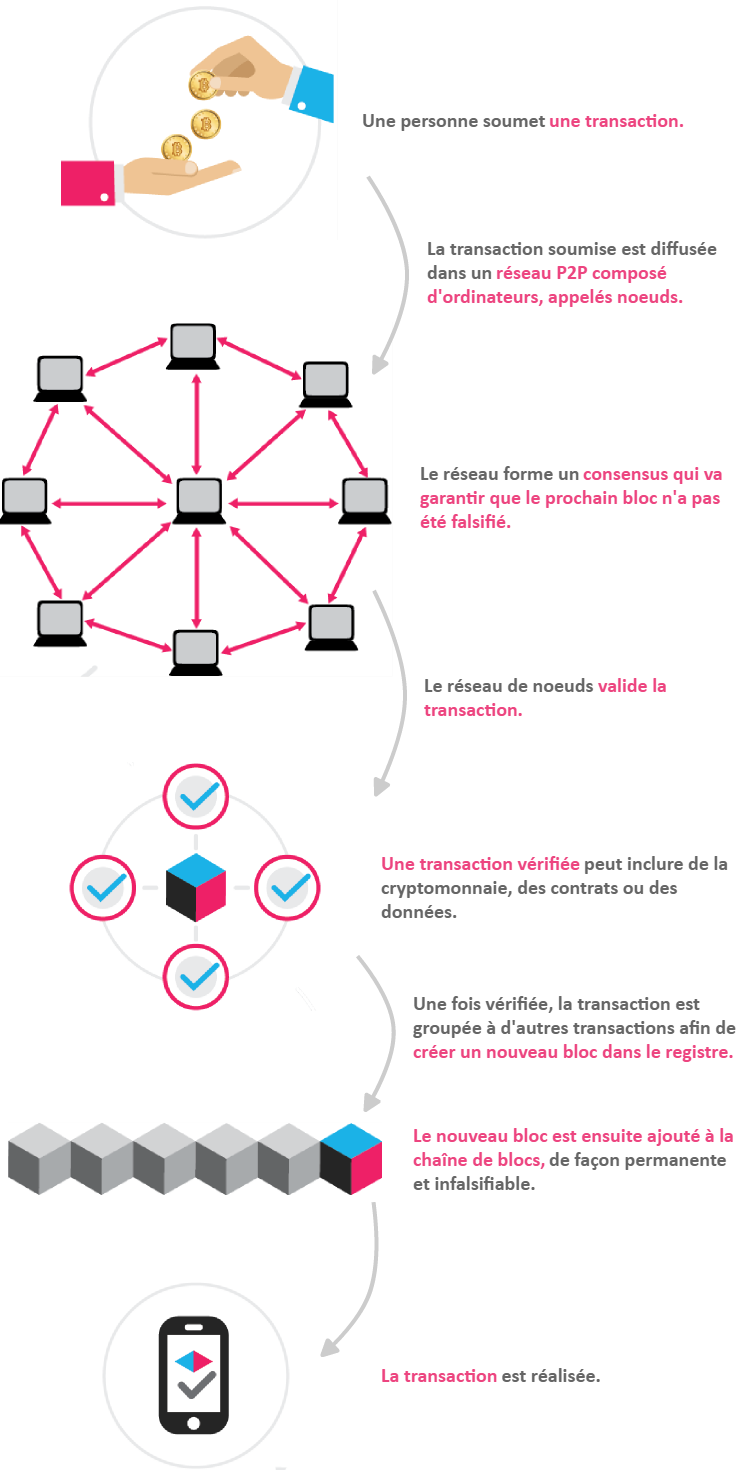
\includegraphics[scale=0.45]{figures/blockchain-diagram}
	\caption{Processus de création est de validation d'une transaction sur la blockchain \cite{blockchain}}
	\label{fig:blockchain-diagram}
\end{figure}
\clearpage

Les blocs de transaction sont agencés dans un ordre linéaire, c'est-à-dire comme une chaîne, et contiennent une référence au bloc précédent, ainsi qu'un enregistrement des transactions.
La preuve de travail est le traitement nécessaire pour générer un nouveau bloc basé sur les nouvelles transactions diffusées sur le réseau.
Les blocs de transaction sont créés par un processus appelé le minage\footnote{mining en anglais.},

http://www.ethdocs.org/en/latest/mining.html

 qui est conçu pour être coûteux en temps et en énergie et pour être complexe à réaliser, et s'appuie sur un consensus pour ajuster la difficulté de créer de nouveaux blocs.

\subsection{Avantages de la blockchain}

Si cette technologie connaît un tel succès c'est parce qu'elle apporte de nombreux avantages : 
\begin{itemize}
	\item la décentralisation, qui signifie que son architecture ne repose pas sur une entité centrale et permet d'enregistrer des données dans un réseau distribué; 
	\item la transparence, puisque l'état des données conservées est consultable publiquement par tout le monde; 
	\item l'autonomie, puisqu'elle est basée sur un consensus dans lequel chaque partie prenante peut transférer des données de manière sécurisée et autonome;
	\item l'immutabilité, en effet toute transaction est persistée définitivement et donc ne peut être effacée;
	\item l'anonymat, car toute personne est anonyme dans le sens où elle n'est pas désignée par son identité mais uniquement par une clé publique\footnote{Une clé publique est un encodage rendu public dans le cadre d'un échange d'informations utilisant le principe de la cryptographie asymétrique.}.
\end{itemize}

\subsection{Inconvénients de la blockchain}

Bien que la blockchain apporte de nombreux avantages, elle comporte aussi des inconvénients :
\begin{itemize}
	\item la performance, en effet cette technologie sera toujours plus lente qu'une base de données centralisée puisqu'elle nécessite pour chaque transaction une vérification de signature, une validation pour le consensus et la redondance des informations; 
	\item la consommation énergétique, puisque la validation de blocs reposent sur la résolution d'un puzzle cryptographique nécessitant une grande puissance de calcul; 
	\item le coût, dans le cas où il est nécessaire d'effectuer un grand nombre de transactions coûteuses;
	\item la confidentialité, puisque toute information enregistrée dans la blockchain est publique, il est fortement déconseillé d'y stocker des informations confidentielles ou personnelles, même si elles sont chiffrées.
\end{itemize}

\subsection{Présentation des Smart Contracts ????}

\section{Définition du cadre et des objectifs du stage}

Dans ce contexte, un stage ingénieur a été réalisé sur une période de 6 mois au sein de la société Arηs Spikeseed située au Luxembourg. 
Le stage a été réalisé dans les locaux de l'entreprise, la langue officielle du projet pour les communications avec les autres membres du consortium (mails, documents, conférence téléphonique) est l’anglais, il en est de même pour la langue utilisée au sein de l'équipe puisque c'est une équipe multinationale. Les documents produits, et présentés dans ce mémoire, ont donc été rédigés en anglais.
Ce stage de fin d'études a pour objectif d'intégrer la technologie blockchain au sein d'un processus de gestion de listes de services de confiance dans le cadre d'un règlement européen. 
La finalité est d'utiliser cette technologie afin de conserver des données publiques relatives à la confiance électronique de manière sécurisée et décentralisée en utilisant une blockchain en tant que registre.
Cela a pour but d'assurer la disponibilité et l'intégrité des informations, puisque les données sont distribuées à travers les nœuds du réseau et sécurisées à l'aide de transactions signées et vérifiées par une preuve mathématique. 

\section{Mise en exergue du plan}

\textbf{ÉDIT EN FONCTION DU PLAN DÉFINITIF}

\textit{
Ce mémoire vise à montrer que le champ d'application de la technologie blockchain dépasse son cadre initial et que son utilisation permet de pallier aux problèmes d'architecture et de sécurité des modèles actuels. 
Dans un premier temps, le contexte du projet sera défini, puis la problématique, qui détaillera les limites des architectures actuelles, sera exposée. 
Ensuite, sera établit un état de l'art afin de comparer les outils existants et de justifier les choix opérés durant le stage. 
Après cela, la réalisation du projet sera développée en expliquant: 
le choix de l'architecture mise en place; 
l'avantage de persister des données dans un système de fichiers décentralisé; 
l'intérêt de gérer l'authentification des utilisateurs par la mise en place d'un consensus; 
l'implémentation d'un système de contrôle de versions et d'un moteur de recherche sur des données stockées dans un réseau décentralisé et distribué. 
Enfin, les résultats obtenus et les perspectives du projet seront détaillés.
}

\chapter{Présentation du contexte}

\section{L'entreprise Ar{\texteta}s Spikeseed}

Ar{\texteta}s Spikeseed est une entité du groupe Ar{\texteta}s qui est une entreprise de services du numérique (ESN) fondée en 2003 par Jourdan Serderidis. 
Le groupe est divisé en sociétés réparties au Luxembourg, en Belgique, en Grèce et depuis cette année en Italie. Le groupe Ar{\texteta}s possèdent cinq axes de compétences qui sont présentés dans la Figure~\ref{fig:arhs-core-services}.

\begin{figure}[h]
	\centering
	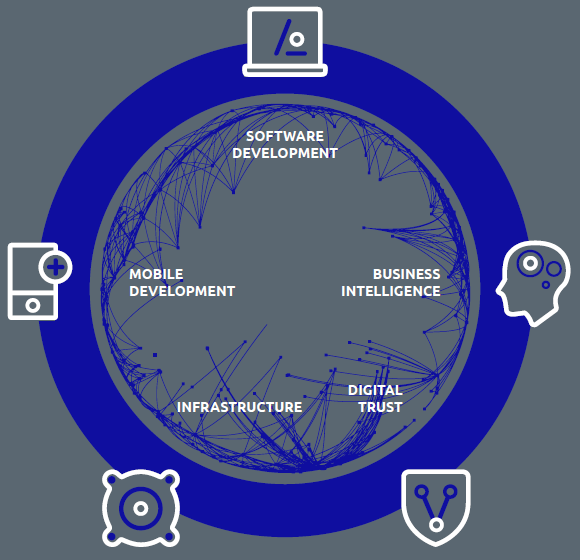
\includegraphics{figures/arhs-core-services}
	\caption{Axes de compétences du groupe Ar{\texteta}s \cite{annual-report}}
	\label{fig:arhs-core-services}
\end{figure}

Comme toutes les autres entités du groupe, Ar{\texteta}s Spikeseed vise à délivrer des solutions numériques complexes. Elle a la particularité de réaliser principalement des projets de recherche et développement en s'appuyant sur les pratiques agiles et des technologies de pointe. 
De plus, Ar{\texteta}s Spikeseed est compétente afin de mettre en œuvre: 
des solutions liées à la confiance numérique; 
des systèmes engageant des masses de données grâce à des technologies innovantes et efficaces comme le Web sémantique ou la Business intelligence; 
des applications destinées aux mobiles et aux objets connectés.

\section{Contexte du projet}

Dans le cadre d'un règlement de l'Union Européenne (UE) sur l'identification électronique (eID) et les services de confiance pour les transactions électroniques sécurisées au sein de l'UE (eIDAS), la Commission Européenne (CE) a émis un appel à projet qui a pour visée de supporter la mise en œuvre technique de ce règlement européen. 
Ce projet de recherche et développement appelé FutureTrust rassemble un consortium de seize partenaires, dont Ar{\texteta}s Spikeseed, engagé dans la réalisation et la mise en application du règlement européen. 
Le projet FutureTrust répondra au besoin de solutions globales et interopérables, en fournissant des logiciels libres qui faciliteront l'utilisation de l'identification et de la signature électronique. 
Il vise à étendre l'infrastructure de la liste européenne de services de confiance existante vers une liste mondiale des services de confiance, nommée Global Trust Service Status List (gTSL), à développer un service de validation ainsi qu'un service d'archivage pour les signatures et les sceaux électroniques, et à fournir des composants pour les certificats qualifiés et pour la création de signatures et de sceaux dans un environnement mobile.

Ce stage de fin d'études a porté sur l'intégration la technologie blockchain dans le cadre du projet FutureTrust et plus particulièrement sur son intégration dans le module de gTSL. Les autres modules du projet ne seront pas détaillés dans ce document. 

\chapter{Présentation détaillée de la problématique}

Les architectures logicielles évoluent en suivant les innovations technologiques. Aujourd'hui, le domaine de la recherche apporte des nouvelles technologies ou des améliorations aux concepts existants à une vitesse exponentielle, si bien que 
le temps de réalisation d'un projet le rend obsolète lors de sa livraison.
Le meilleur exemple de ce phénomène est le framework Angular, initié par Google, qui est passé de la version 2 à la version 5 en moins d'une année. C'est la réalité actuelle de l'univers technologique poussé par l'innovation, un monde où les acteurs doivent s'adapter en permanence aux changements. La technologie blockchain s'inscrit dans ces innovations récentes issues de la recherche. Elle amène une nouvelle vision d'un Internet décentralisé sans organe central de contrôle, qui va probablement révolutionner la conception des systèmes d'information dans les prochaines années. Dans ce contexte, l'utilisation de la blockchain a été proposée dans le cadre du projet FutureTrust.

\section{Description du service de liste de confiance globale}
\label{sec:description}

Les États membres de l'UE et d'autres pays européens maintiennent généralement des listes d'autorités de certification et d'autres fournisseurs de services de confiance, désignés Trust Service Providers (TSP), dans un ou plusieurs registres à l'échelle nationale.
La liste de confiance des États membres de l'UE comprend des informations relatives aux TSPs qualifiés qui sont supervisés par l'État membre compétent, ainsi que des informations relatives aux services de confiance, désignés Trust Services (TS), qu'ils fournissent, conformément aux dispositions prévues par le règlement eIDAS.
Les listes de confiance sont des éléments essentiels dans la mise en place de la confiance numérique pour les opérateurs du marché électronique, en permettant aux utilisateurs de déterminer le statut qualifié des TSPs et de leurs TSs. En vertu du règlement eIDAS, les listes nationales de confiance ont un effet constitutif.
En d'autres termes, un fournisseur ou un service ne sera qualifié que s'il apparaît dans les listes de confiance. Par conséquent, les utilisateurs (citoyens, entreprises ou administrations publiques) bénéficieront de l'effet juridique associé à un service de confiance qualifié donné uniquement si ce dernier est répertorié (comme qualifié) dans les listes de confiance.	
Les États membres peuvent inclure dans les listes de confiance des informations sur les fournisseurs de services de confiance non qualifiés et sur d'autres services de confiance définis au niveau national.

La structure d'une liste de confiance est présentée dans la Figure~\ref{fig:tsl-scheme}.

\begin{figure}[h]
	\centering
	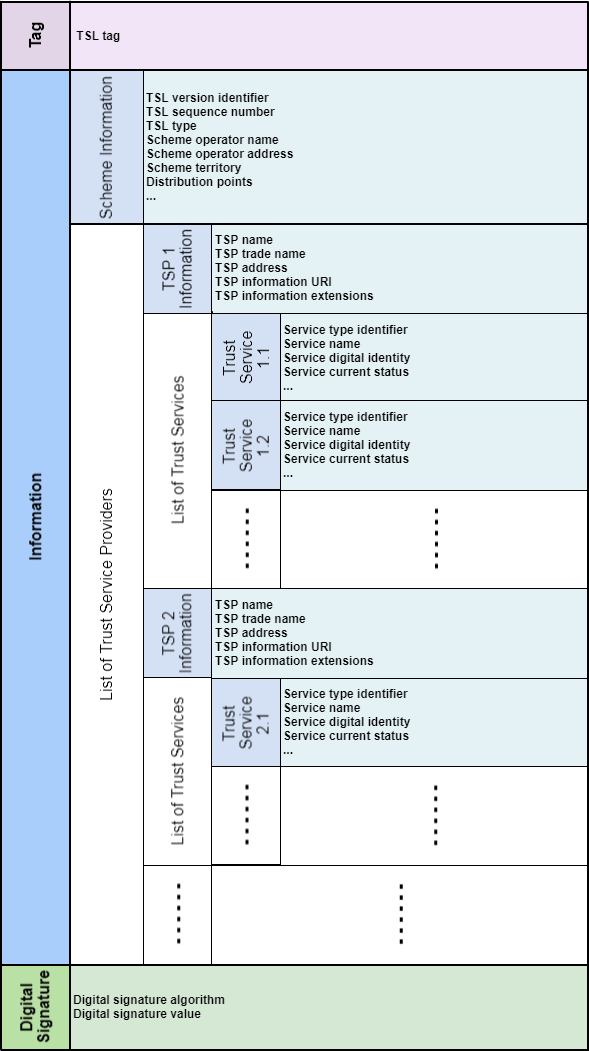
\includegraphics[scale=0.65]{figures/tsl-scheme}
	\caption{gTSL – Structure d'une liste de confiance}
	\label{fig:tsl-scheme}
\end{figure}

\clearpage

Dans la Figure~\ref{fig:tsl-scheme}, on distingue qu'une liste de confiance peut être décomposée en trois sections. 

\subsubsection{Tag}

La section \textit{Tag}, et plus particulièrement son attribut \textit{TSL Tag}, est une URI\footnote{Une URI (acronyme anglais de Uniform Resource Identifier) est une chaîne de caractères identifiant une ressource.} qui permet d'indiquer le standard respecté par la liste de confiance. Actuellement, le seul standard  existant est ETSI TS 119 612~\cite{ETSITS119612}. Il est possible qu'un nouveau standard soit défini dans le futur, cette section permettra donc d'indiquer le standard sur lequel la liste de confiance est basé.

\subsubsection{Information}

La section \textit{Information} peut-être divisée en deux parties. 
La première partie, nommée \textit{Scheme Information}, répertorie toutes les informations relatives à la liste de confiance comme par exemple sa version, le nom et l'adresse de l'opérateur de la liste ou encore le pays pour lequel la liste est définie. Il est important de noter que dans la Figure~\ref{fig:tsl-scheme} la liste des informations n'est pas exhaustive. 
La seconde partie est la liste des TSPs qui répertorie l'ensemble des fournisseurs approuvés par l'État membre. Pour chacun des TSPs, on retrouve ses informations ainsi que la liste des services de confiances qu'il fournit.

\subsubsection{Digital Signature}

La section \textit{Digital Signature} permet de vérifier l'authenticité et l'intégrité de la liste de confiance. En effet, chaque liste doit être signée par l'opérateur prévu à cet effet, défini dans la partie \textit{Scheme Information}. Dans cette section doit être indiquée la signature de l'opérateur ainsi que l'algorithme de génération de celle-ci.

\subsection{Besoins générales}

\subsubsection{Intérêt du projet}

L'intérêt d'un service de 
%liste mondiale des services de confiance 
gTSL 
est de favoriser l'établissement de relations de confiance entre les opérateurs du marché en Europe et au-delà. À ce titre, elle étend le schéma actuel de la liste des services de confiance, dont la portée est uniquement européenne. Cette liste a pour but de répertorier les TSPs, ayant un statut qualifié ou non. On entend par statut qualifié que le TSP ait été accrédité par un organisme compétent au sein de l’État membre dans lequel le TSP est déclaré. Le service permet aux utilisateurs finaux de vérifier le statut de ces TSPs et d'accéder à l'ensemble des informations concernant les services de confiance.

%The business purpose of the Global Trust Status List Service specified in the present document is to foster the building of trust relationships between market operators across Europe, and beyond. As such, it extends the current Trust Status List scheme which indicates whether Trust Service Providers have a qualified status or not.

%\subsubsection{Stakeholders}
\subsubsection{Parties prenantes}

Les acteurs principaux de la 
%liste mondiale des services de confiance
gTSL
sont:
\begin{itemize}
	\item les États membres de l'UE, qui doivent établir, maintenir et publier les listes de confiance, incluant les informations relatives aux TSPs de services déclarés au sein de leur État;
	\item les fournisseurs de services de confiance, qui sont destinés à s'appuyer sur le service de gTSL dans lequel sont publiés leur statut qualifié et leurs informations publiques;
	\item les opérateurs de liste de confiance ne faisant pas partie d'un État membre de l'UE, qui souhaitent intégrer leur liste dans la gTSL;
	\item les citoyens de l'UE et non UE, qui sont destinés à utiliser le service afin d'accéder aux statuts et aux informations des différents TSPs répertoriés dans la gTSL.
\end{itemize}

%\subsubsection{Goal and Objective}
\subsubsection{Objectif du projet}

L'objectif principal de la gTSL est de gérer et de fournir les informations relatives aux TSPs qualifiés au sein de l'Union Européenne et au-delà, en étendant le modèle actuel de la liste européenne de services de confiance. De plus, cette réorganisation de l'architecture vise à gérer la gTSL de manière décentralisée dans le but d'en améliorer sa résilience ainsi que sa gestion.

\subsection{Besoins du système}
\label{sec:system-requirements}

\subsubsection{Objectif du système}

En s'appuyant sur la norme de listes de confiance définie dans ETSI TS 119 612~\cite{ETSITS119612}, la gTSL vise à résoudre les imperfections actuelles du schéma de liste de confiance, énoncées dans la Section~\ref{sec:limits}, lorsqu'il est considéré dans un contexte globalisé. 
À l'heure actuelle, la Commission européenne publie une liste signée de pointeurs, nommée European List of the Lists (LoTL), dans laquelle chaque pointeur désigne un point de distribution pour une liste nationale de TSPs. 
Ces listes nationales contiennent des informations sur les TSPs qualifiés et non qualifiés ainsi que sur les services qualifiés ou non qualifiés qu'ils proposent.

\subsubsection{Portée du système}

La portée de la gTSL concerne la définition de services de confiance qualifiés et de fournisseurs de services de confiance.
À ce titre, elle fournira les fonctions nécessaires à la création, à la mise à jour et à la distribution des fournisseurs de services de confiance et des informations concernant leurs services de confiance.

\subsubsection{Présentation du système}

Afin d'atteindre ses objectifs, le gTSL s'appuiera sur deux principaux composants open source:
\begin{itemize}
	\item Global Trust Service Lifecycle Manager\footnote{en français, Gestionnaire du cycle de vie.}
	\item Global Trust Service Responder\footnote{en français, Répondeur (dans le sens où il répond aux requêtes des utilisateurs).}
\end{itemize}
De plus, la gTSL s'appuiera sur une interface d'administration afin de présenter les fonctions de gestion des listes de confiance aux utilisateurs.
Ces composants et leurs interactions sont illustrés dans la Figure~\ref{fig:3tier-archi}.

\begin{figure}[h]
	\centering
	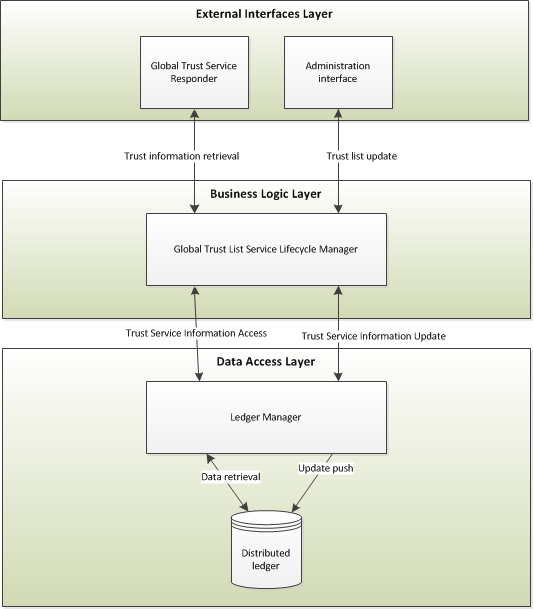
\includegraphics{figures/gTSL-3Tier}
	\caption{gTSL – Architecture 3-Tier \cite{design-document}}
	\label{fig:3tier-archi}
\end{figure}

%\clearpage

L'objectif du Global Trust Service Responder est de permettre aux applications externes et aux utilisateurs d'interroger la gTSL afin de récupérer les informations relatives aux TSPs, dans le but de vérifier leur statut à un moment donné. 
Il fournira donc les fonctions nécessaires pour répondre aux demandes d'information sur les statuts de confiance.
L'objectif du Global Trust Service Lifecycle Manager est de faciliter la gestion de la hiérarchie des services de confiance, et de permettre la mise à jour du statut des TSPs.
Il fournira les fonctions nécessaires à la création, à la mise à jour et à la distribution des informations relatives aux statuts de confiance.

D'un point de vue architectural, le gTSL s'appuiera sur une architecture à 3 couches:
\begin{itemize}
	\item La couche de services externes exposera les interfaces externes du système, i.e. le Global Trust Service Responder et l'interface d'administration;
	\item La couche métier sera composée du Global Trust List Service Lifecycle Manager;
	\item La couche de données correspondra aux interfaces et aux composants qui permettent de connecter le gTSL à une solution de stockage de données.
\end{itemize}
L'un des objectifs de la gTSL est de s'appuyer sur le modèle de distribution centralisé actuel et de l'adapter à un nouveau modèle décentralisé.
L'émergence récente du concept de blockchain et les développements qui l'accompagnent dans les solutions de stockage de données basé sur cette technologie apportent un ensemble de solutions potentielles à cet objectif de décentralisation.

La Section~\ref{sec:state-of-the-art} présente les différentes implémentations de blockchain et de système de stockage de données décentralisé pouvant s'interfacer avec une blockchain qui ont été considérées et décrit les interfaces définies pour la couche de données.

\subsubsection{Contexte du système}

La Figure~\ref{fig:system-context-diagram} fournit une description de haut niveau des interactions du système avec des entités externes.

\begin{figure}[h]
	\centering
	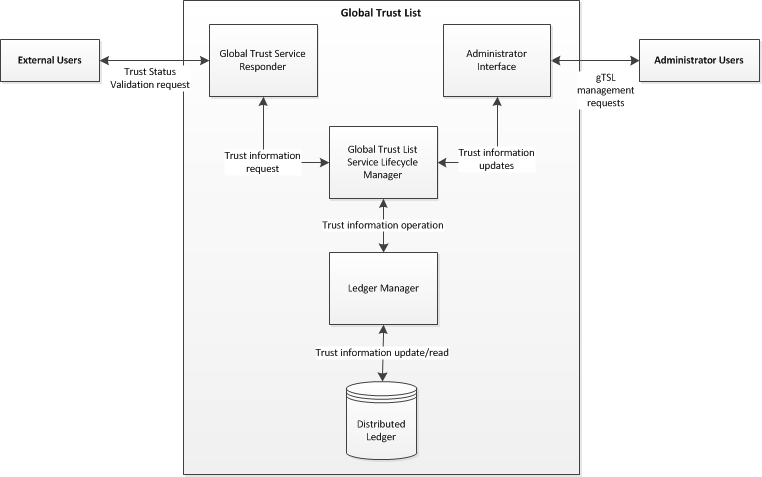
\includegraphics[scale=0.8]{figures/gTSL-SystemContextDiagram}
	\caption{gTSL - Schéma du contexte du système \cite{design-document}}
	\label{fig:system-context-diagram}
\end{figure}

L'entité External Users\footnote{en français, utilisateurs externes.} représente tous les utilisateurs externes qui souhaitent interagir avec le système sans privilège spécifique, dans le but de récupérer des informations relatives à la gTSL. Le Validation Service\footnote{en français, service de validation.} développé dans le cadre du projet FutureTrust est un des ces utilisateurs externes.
L'entité Administrator Users\footnote{en français, utilisateurs d'administration.} représente tous les utilisateurs externes qui sont autorisés à effectuer des opérations de gestion sur la gTSL, comme par exemple mettre à jour les informations d'un TSP.

\subsubsection{Caractéristiques des utilisateurs}

Deux types différents d'utilisateurs ont été identifiés concernant la gTSL:
\begin{itemize}
	\item Utilisateurs d'administration, i.e. les administrateurs de plates-formes, qui peuvent agir au nom d'un État membre de l'UE et qui sont chargés de la maintenance quotidienne et de la gestion des listes de confiance;
	\item Utilisateurs externes, i.e. les personnes et les applications externes qui souhaitent obtenir des informations concernant les statuts de confiance pour un TSP, un TS ou un État membre donné.
\end{itemize}

Ces utilisateurs auront accès au système à travers des interfaces dédiées:
\begin{itemize}
	\item Utilisateurs d'administration auront accès à une plateforme de gestion de la gTSL, qui exposera sans ambiguïté les différentes fonctionnalités d'administration auxquelles les utilisateurs doivent avoir accès;
	\item Utilisateurs externes auront accès à la fois à une interface graphique et à une seconde interface de web services\footnote{Un web service correspond à l'implémentation d'une ressource identifiée par une URL.}, qui permettra la récupération d'informations concernant les statuts des services de confiance sur base de certificats électroniques fournis par l'utilisateur ainsi que des informations générales concernant les TSPs.
\end{itemize}

\subsubsection{Besoins fonctionnelles}

Les besoins fonctionnelles identifiés pour la gTSL sont:
\begin{itemize}
	\item La gTSL doit permettre la gestion des {\em Trust Anchors and Meta-data of Identity Providers;}
	\item La gTSL doit supporter l'internationalisation (non-UE) du règlement eIDAS. À ce titre, la gTSL doit permettre l'ajout de TSPs déclarés dans un pays qui n'est pas membre de l'UE, qu'ils soient qualifiés ou non.
\end{itemize}

\subsubsection{Besoins d'utilisation}

Les besoins d'utilisation identifiés pour la gTSL sont:
\begin{itemize}
	\item La gTSL doit offrir une interface permettant la récupération ainsi que la publication d'informations relatives aux TSPs. Au minimum, afin d'assurer la conformité avec le standard ETSI TS 119 612~\cite{ETSITS119612}, la gTSL doit être disponible via le protocole HTTP.
\end{itemize}

\subsubsection{Besoins de performance}

Les besoins de performance identifiés pour la gTSL sont:
\begin{itemize}
	\item la gTSL doit apporter un stockage interne efficace pour stocker les informations de statut sur les TSPs.
	\item la gTSL doit être hautement scalable afin de gérer efficacement de nombreuses quantités de demandes parallèles.
\end{itemize}

\subsubsection{Interfaces du système}

La gTSL doit exposer, grâce à une interface de web services, les fonctionnalités permettant la récupération d'informations concernant les statuts des services de confiance.

\subsubsection{Interfaces utilisateurs}

Les fonctionnalités de gestion de la gTSL doivent être fournies à travers une interface web cohérente et intuitive, permettant aux utilisateurs de l'utiliser sans ambiguïté. 
Les interfaces utilisateur doivent rester cohérentes avec les interfaces utilisateur de l'application TL-Manager actuelle tout en ne montrant aucune ambiguïté en termes de hiérarchie visuelle et de contenu.

\subsubsection{Fiabilité du système}

La gTSL doit être disponible sur une base de 24 heures par jour et 7 jours par semaine.
Plus particulièrement, dans le but d'être conforme avec le standard ETSI TS 119 612~\cite{ETSITS119612}, le Global Trust Service Responder doit être disponible sur une base de 24 heures par jour et 7 jours par semaine, avec une disponibilité annuelle minimum de 99.9\%.

\subsubsection{Sécurité du système}

En raison de la nature sensible des données gérées par la gTSL, et de la haute disponibilité requise, les besoins en terme de sécurité doivent garantir que ces données ne peuvent être et ne sont pas compromises et que la gestion des services de confiance et des fournisseurs de services de confiance est clairement limitée aux personnes autorisées.
La gTSL ne doit pas permettre à des personnes non autorisées de créer, modifier ou supprimer des informations relatives à des services de confiance ou des fournisseurs de services de confiance.
La gTSL doit assurer l'intégrité des données qu'elle traite.

\subsection{Besoins logicielles}

\subsubsection{Conformité au standard}

La gTSL doit être conforme avec le standard ETSI TS 119 612~\cite{ETSITS119612}. À ce titre, la gTSL doit respecter:
\begin{itemize}
	\item le format et la sémantique d'une liste de confiance;
	\item les mécanismes à utiliser pour aider les parties prenantes à localiser, à accéder et à authentifier les listes de confiance.
\end{itemize}

\subsubsection{Rétrocompatibilité}

La gTSL doit pouvoir s'intégrer au schéma existant basé sur la LoTL. Cela signifie qu'elle est capable d'importer l'ensemble des listes de confiance actuellement référencées dans la LoTL, mettre en évidence les changements au fur et à mesure qu'ils se produisent grâce à un historique et permettre d'ajouter d'autres TSPs hors UE.

\section{Limites de l'architecture actuelle}
\label{sec:limits}

Avec le modèle actuel, les modifications apportées au contenu d'une liste nationale induisent la nécessité de republier toute la liste nationale. De plus, toutes modifications apportées sur l'URL\footnote{Une URL (acronyme anglais de Uniform Resource Locator) est couramment appelé adresse web.} à laquelle la liste est distribuée ou sur le certificat utilisé pour signer la liste, induisent la nécessité de republier à la fois la liste nationale et la liste européenne.
Le caractère centralisé du système de distribution des listes de confiance actuel contient des potentiels problèmes qui doivent être résolus dans le cadre de la globalisation des listes de services de confiance:
\begin{itemize}
	\item les listes de confiance des États membres sont uniquement récupérable en se basant sur la LoTL, le schéma actuel est donc sujet à un point individuel de défaillance\footnote{Un point individuel de défaillance (single point of failure ou SPOF en anglais) est un point d'un système informatique dont le reste du système est dépendant et dont une panne entraîne l'arrêt complet du système.};
	\item chaque État membre maintient les données relatives à sa liste de confiance, cela signifie que l'arrêt du nœud de distribution d'un État membre rend ses données non consultables;
	\item l'architecture existante est exposée à un problème de résilience puisqu'elle nécessite que l'ensemble des nœuds de distribution des États membres soit actifs afin que la liste globale soit considérée complète et donc fiable;
	\item l'intégrité des données peut être compromise, en effet si les données d'un État membre sont corrompues localement sur son nœud de distribution, alors l'intégrité globale est compromise puisqu'on se fie uniquement à ce nœud de distribution;
	\item des problèmes de performance et de latence peuvent être rencontrés puisqu'il est nécessaire de télécharger et valider l'ensemble des informations qui sont réparties sur différents points de distribution;
	\item le schéma actuel ne conserve pas l'historique des modifications, c'est-à-dire qu'une nouvelle publication d'une liste remplace totalement la précédente, ce qui ne permet pas de conserver une trace des modifications mises en œuvre entre les versions;
\end{itemize}

L'objectif de la gTSL est d'effectuer une refonte de l'architecture actuelle qui a montré ses limites en y apportant des technologies innovantes. Pour cela, il est nécessaire d'adopter un modèle décentralisé et distribué qui permettra de résoudre les problèmes de résilience et de point individuel de défaillance. La technologie blockchain apporte en plus des avantages qui permettront de s'assurer de l'intégrité des données ainsi que de la sécurité du système.

\section{Gestion de projet}

\subsection{Méthode de gestion de projet}

La méthode Agile a été utilisée au cours de ce projet. 
Plus particulièrement, l'équipe s'est appuyée sur le schéma Scrum, qui permet un cadre de travail itératif où les tâches majeures sont décomposées en sous-tâches.
La méthodologie Scrum est basée sur le découpage d'un projet en sprints\footnote{Un sprint est une période sur laquelle sont réalisées des tâches définies.}, qui sont des cycles de livraison très courts.
Un sprint peut s'étendre sur une durée de quelques heures à un mois. 
Dans notre cas, nous avons choisi une durée de deux semaines par sprint.
En début de sprint, une estimation de la durée de chaque tâche est effectuée, ensuite une planification opérationnelle est réalisée.
Un sprint se termine généralement par une démonstration du travail réalisé suivie d'une rétrospective, afin d'analyser le déroulement du sprint achevé et dans le but d'améliorer les pratiques de l'équipe. 
Quotidiennement est organisé un scrum meeting\footnote{Un scrum meeting est communément appelé mêlée en français.}, réunion courte et énergique, qui permet à l'équipe de discuter de l'avancée du sprint et de lever les points bloquants du projet.
Afin de suivre la progression des objectifs au fur et à mesure de l’avancement du projet, nous avons utilisé l'outil JIRA. Il a servi notamment à définir les différentes tâches du projet et à répartir le travail entre les membres de l’équipe.

\subsubsection{Les avantages majeures de Scrum}

Scrum apporte des avantages qui sont définies comme étant les trois piliers de la méthodologie:
\begin{itemize}
	\item la transparence, par l'utilisation d'un langage commun afin de permettre à tout un chacun d'obtenir rapidement une bonne compréhension du projet et par la garantie que tous les indicateurs relatifs à l’état du développement soient visibles; 
	\item l'inspection, par l'analyse quotidienne du travail accompli et restant lors des sprints, afin de repérer tout indicateur indésirable;
	\item l'adaptation, dans le cas d'une dérive après inspection, des ajustements doivent être effectués afin de minimiser les écarts de réalisation.
\end{itemize}

\subsection{Organisation du temps}

La Figure~\ref{fig:gantt} est un diagramme de Gantt qui expose de manière globale la répartition du travail réalisé. Ce diagramme est volontairement non détaillé puisque l'utilisation de la méthodologie Agile ne permet pas d'organiser à l'avance et avec précision la réalisation des tâches. Il est important de noter que le diagramme se termine à la date de fin du stage mais que la livraison du projet est prévue au 30 novembre 2017.

\begin{figure}[h]
	\centering
	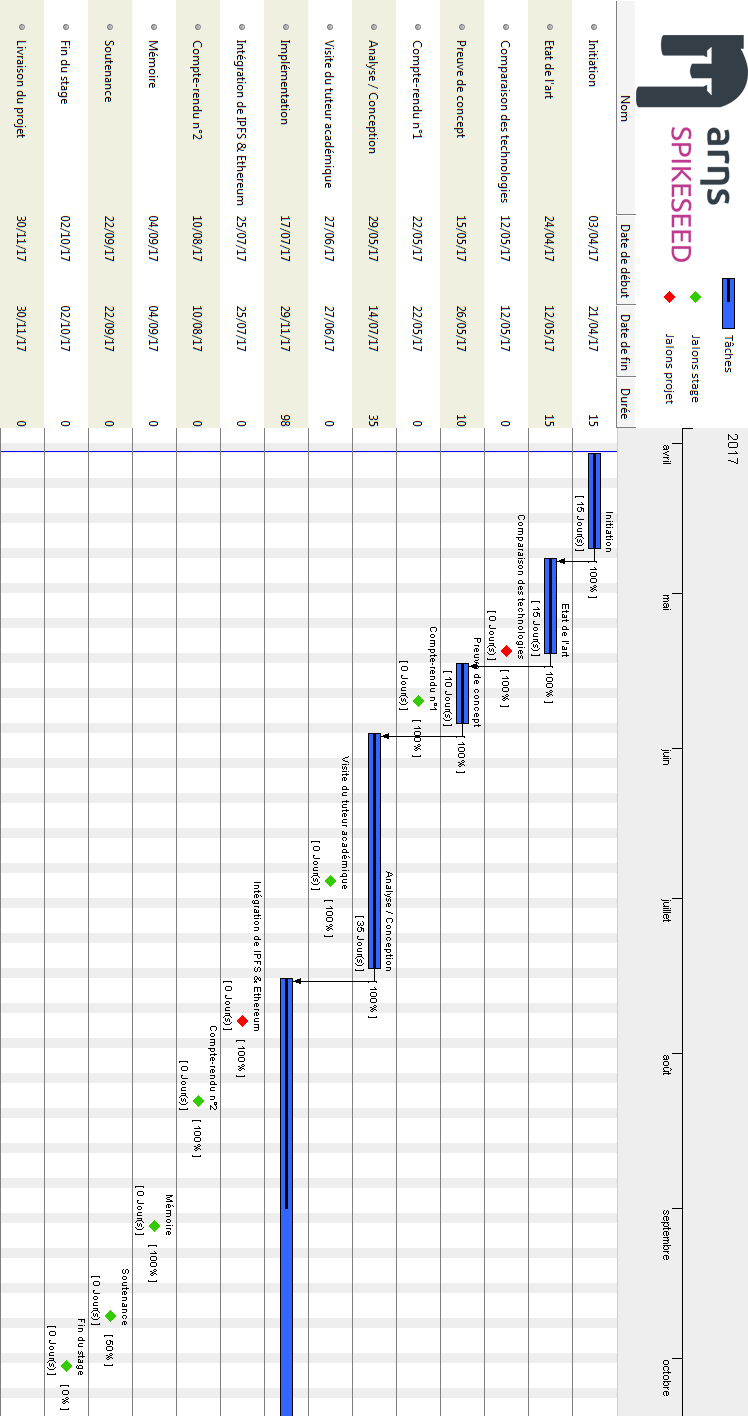
\includegraphics[scale=0.67]{figures/gantt-stage-vertical}
	\caption{Diagramme de Gantt}
	\label{fig:gantt}
\end{figure}

\clearpage

Le diagramme de Gantt en Figure~\ref{fig:gantt} permet d'avoir un aperçu de l'organisation du stage. Le stage s'est déroulé sur une période de six mois, du 3 avril 2017 au 30 septembre 2017. Durant cette période, j'ai été amené à réaliser différentes tâches qui seront détaillées dans la suite de ce mémoire. D'un point de vue générale, le stage a été décomposée en cinq parties majeures qui sont décrites ci-après.

\subsubsection{Initiation}

La phase d'initiation a commencé dès le début du stage et a duré environ trois semaines. 
Elle peut être décomposée en deux sous-parties. Dans un premier temps, j'ai dû me familiariser avec le projet. Pour réaliser cela, j'ai eu accès au document de conception de la gTSL~\cite{design-document} qui explique, d'une manière générale et sans précision de technologies, l'architecture à mettre en place ainsi que les cas d'utilisation à implémenter dans le cadre du projet FutureTrust. J'ai pris connaissance du standard ETSI TS 119 612~\cite{ETSITS119612} qui détaille le format à respecter dans le cadre des listes de confiance. Dans un second temps, j'ai effectué des recherches sur les notions de cryptographie, de signature électronique et de blockchain afin de les mettre en œuvre dans le projet. Cette seconde partie a été la préparation du travail suivant qui est l'état de l'art.

\subsubsection{État de l'art}

La seconde phase, ayant pour objectif d'établir un état de l'art, a suivi la phase d'initiation et s'est étendue sur trois semaines.
L'état de l'art permet de connaître l'état des connaissances et technologies actuelles dans un domaine spécifique. Pour notre projet, l'état de l'art a porté sur la blockchain ainsi que les systèmes de stockage de données décentralisés. Le but de cette phase a été d'explorer le plus largement possible les technologies pouvant être utilisées dans le projet afin de les comparer et de choisir les solutions répondant à nos besoins. Cette étape a donné lieu à un livrable qui a été inclus dans le document de conception de la gTSL comme le montre le jalon "Comparaison des technologies" dans la Figure~\ref{fig:gantt}. L'état de l'art est détaillé dans la Section~\ref{sec:state-of-the-art}.

\subsubsection{Preuve de concept}

À la suite de l'état de l'art, un choix de technologies a été effectué. L'étape suivante a donc été de prouver que les choix opérés correspondent aux besoins du projet. Pour cela, j'ai pu réaliser une preuve de concept sur une durée de quinze jours. Cette phase a ensuite donné lieu à une démonstration à l'équipe afin de valider de manière définitive les choix technologiques. Le détail de la preuve de concept ainsi que la justification des choix opérés sont présentés dans la Section~\ref{sec:realisation}.

\subsubsection{Analyse / Conception}

La phase d'analyse et conception a été précédée de la preuve de concept qui a permis de valider les technologies à utiliser pour le projet. Dans le cadre de cette phase, nous avons déterminé les modules à implémenter afin de répondre aux besoins exprimés dans le document de conception. L'analyse et la conception ont consisté à réfléchir sur la mise en place d'une architecture décentralisée basée sur une blockchain en étant conforme aux différentes contraintes définies dans le document de conception et en s'appuyant sur les technologies choisies. Cette partie a duré un mois et demi, et est détaillée dans la Section~\ref{sec:analyse}.

\subsubsection{Implémentation}

La dernière phase, et la plus conséquente puisqu'elle s'étend sur de la mi-juillet à fin novembre, est l'implémentation. Elle consiste à développer la solution conçue et imaginée lors de la phase d'analyse et conception. Lors de la rédaction de ce mémoire, cette phase est en cours de réalisation. Cette phase est découpée en sprints d'une durée chacun de deux semaines. L'implémentation est détaillée dans la Section~\ref{sec:realisation}. 

\chapter{État de l'art}
\label{sec:state-of-the-art}

S'INSPIRER DU WHITE PAPER ETHEREUM

\begin{itemize}
	\item On veut une techno pour stocker, gérer et récupérer les données de la gTSL; 
	\item Amener sur le type de techno à utiliser (blockchain, database décentralisée, file system décentralisé...);
	\item Enoncer le principal désavantages de la blockchain qui est son coût (cf. Ethereum \& IPFS integration);
	\item Validation par une preuve de concept
\end{itemize}

\section{L'émergence de la blockchain}

\section{La décentralisation du web}

\section{Solutions existantes}

La couche de persistance des données de la gTSL repose sur la blockchain et des concepts de décentralisation. À ce titre, l'objectif est de conserver toutes les informations relatives aux TSPs et aux TSs dans un registre sécurisé, c'est-à-dire dans une liste chaînée de transactions signées, et de répliquer toutes les données de la gTSL à travers un réseau pair-à-pair\footnote{Le pair-à-pair est un modèle de réseau informatique similaire au modèle client-serveur mais où chaque client est aussi un serveur.} décentralisé.
Cela permet de garantir à la fois l'intégrité et la disponibilité des informations, puisque chaque chaque donnée est signée avec toutes les données précédentes dans le registre. La distribution de l'information à travers un réseau pair-à-pair fournit une résilience forte contre les attaques par déni de service.

Afin d'atteindre cet objectif qui permettra de pallier aux problèmes de l'architecture actuelle, plusieurs options ont été envisagées :
\begin{itemize}
	\item Stocker les données directement dans une blockchain publique existante;
	\item Stocker les données dans une blockchain privée;
	\item Stocker les données dans une blockchain privée, et utiliser une blockchain publique pour s'assurer de l'intégrité des données (par exemple en conservant le hash\footnote{Un hash est le résultat d'une fonction de hachage qui permet d'identifier rapidement une donnée.} de la transaction réalisée sur la blockchain privée dans une blockchain publique);
	\item Stocker les données dans un système décentralisé et distribué, comme par exemple une base de données ou un système de fichiers, et utiliser une blockchain publique pour s'assurer de l'intégrité des données (par exemple en conservant le hashes\footnote{Le terme hashes est le pluriel du mot hash.} ou les références des données).
\end{itemize}

Cette section présente les technologies qui ont été envisagées en tant que solutions de stockage de données dans le cadre de l'implémentation de la gTSL. On y retrouve des technologies de blockchain, mais aussi des systèmes décentralisés et distribués.

\subsection{Ripple}

Ripple\footnote{Voir \url{https://ripple.com/}} est une crypto-monnaie s'appuyant sur un registre distribué basé sur une blockchain qui n'utilise pas de système de preuve de travail pour l'ajout de blocs. Au lieu de cela, il repose sur un mécanisme de consensus (The Ripple Protocol Consensus Algorithm, 2014) appliqué à un sous-réseau de nœuds connus et fiables.

\subsection{Tendermint}

Tendermint\footnote{Voir \url{https://tendermint.com/}} est une crypto-monnaie s'appuyant sur un registre distribué basé sur une blockchain qui utilise un système de votes par un consensus au lieu du minage. À ce titre, Il repose sur un ensemble de nœuds de validation qui sont responsables d'émettre des votes signés pour, ou contre, l'ajout de nouveaux blocs dans la chaîne. Le scrutin est validé si au minimum les deux tiers des nœuds de validation votent pour l'acceptation d'un nouveau bloc.

\subsection{Ethereum}

Ethereum\footnote{Voir \url{https://ethereum.org/}} est une plate-forme publique décentralisée et distribuée basée sur la technologie blockchain. Il repose sur des programmes qui ont leur code (leurs fonctions) et leurs données (leur état) stockés sur la blockchain. Ces programmes s'appellent smart contracts. 
Il apporte donc l'utilisation de concepts de blockchain au-delà du cas d'utilisation de la crypto-monnaie et offre un environnement d'exécution virtuel qui peut être utilisé pour créer des organisations autonomes décentralisées, c'est-à-dire des organisations qui sont gérées par des règles spécifiées dans des smart contracts. Ethereum étant conçu principalement comme un environnement d'exécution décentralisé et autonome, il n'offre pas de fonctionnalités de stockage réelles. Bien que les données puissent être stockées dans le cadre de l'exécution des contrats intelligents, le coût peut rapidement devenir prohibitif. En effet, le système est conçu pour calculer le coût des transactions en fonction des ressources nécessaires en termes de calcul, de bande passante et de stockage. L'intention du système de redevances est d'obliger un attaquant à payer proportionnellement pour chaque ressource qu'ils consomment.

\subsection{Swarm}

Swarm\footnote{Voir \url{http://swarm-gateways.net/bzz:/swarm-gateways.eth/}} est une plate-forme de stockage distribué ainsi qu'un service de distribution de contenu directement lié à Ethereum. Son objectif initial est de servir de solution de stockage décentralisé et redondant pour les enregistrements dans le registre publique d'Ethereum, mais il peut également être utilisé comme une solution de stockage et de service pair à pair. Au moment de la rédaction de ce mémoire, Swarm était encore à ses débuts de développement, avec uniquement une version "alpha" disponible.

\subsection{Hyperledger Fabric}

Hyperledger Fabric\footnote{Voir \url{https://www.hyperledger.org/projects/fabric}} est une plate-forme de registre distribué destinée à l'exécution de smart contracts. Il est conçu avec une architecture modulaire, prend en charge les contrats intelligents écrit dans le langage de programmation Go et repose sur un réseau de pairs de validation (c'est-à-dire les nœuds responsables du maintien du registre) et des pairs de non validation. À l'instar d'Ethereum, Hyperledger ne gère pas le stockage de données nativement et simplement, mais son architecture modulaire pourrait le permettre.

\subsection{Keyless ledger}

Keyless Signature Infrastructure\footnote{Voir \url{https://guardtime.com/technology/ksi-technology}} (KSI) est une plate-forme offrant une authentification basée sur la signature électronique pour les données numériques, les machines et les humains. KSI repose uniquement sur les fonctions de hachage, son registre agit comme un enregistrement de logs\footnote{Le logging est un dispositif permettant de stocker un historique des évènements attachés à un processus.} de timestamps\footnote{Le timestamping, aussi nommé horodatage en français, est un mécanisme qui consiste à associer une date et une heure à un événement, une information ou une donnée informatique.} émis pour les hashes de données soumises par les utilisateurs.

\subsection{OpenChain}

OpenChain\footnote{Voir \url{https://www.openchain.org/}} est un registre distribué open-source qui repose uniquement sur une signature électronique qui est générée pour les transactions qu'il enregistre. Les transactions sont directement liées les unes aux autres, sans l'utilisation de blocs, et peuvent maintenir des données. OpenChain peut posséder plusieurs instances, chacune répliquant les autres. Cependant, la technologie est construite autour d'une hiérarchie de nœuds de validation et de nœuds d'observation, dans laquelle les nœuds de validation peuvent ajouter et valider des transactions pour le registre et les nœuds d'observation peuvent uniquement répliquer les données des nœuds de validation auxquelles ils sont connectés. Par conséquent, il n'est pas possible d'implémenter un réseau purement décentralisé d'instances OpenChain.

\subsection{BigchainDB}

BigchainDB\footnote{Voir \url{https://www.bigchaindb.com/}} aims at linking the database and block-chain worlds by adding block-chain characteristics such as decentralisation, data immutability and asset transfer to existing NoSQL database implementations.
It is however still in its early stages of development and currently lacks basic security controls (e.g. a database administrator deleting a database on one node will see this operation being replicated across all other nodes). Additionally, BigChainDB is not Byzantine Fault Tolerant.

\subsection{InterPlanetary File System (IPFS)}

The InterPlanetary File System\footnote{Voir \url{https://ipfs.io/}} is “a peer-to-peer distributed file system that seeks to connect all computing devices with the same system of files […]” (Benet, 2014).
IPFS re-uses block-chain paradigms such as data immutability and decentralisation achieved through peer-to-peer communication, while basing itself on the Git\footnote{Voir \url{https://ripple.com/}} version control system.

\subsection{Monax}

Monax\footnote{Voir \url{https://monax.io/}} is an open platform aimed at developers that are willing to build and run block-chain based applications for business ecosystems.
As such it can be compared with Ethereum, however with permissions that make it legally usable in business environments.

\subsection{Factom}

Factom\footnote{Voir \url{https://www.factom.com/}} (Factom - Business Processes Secured by Immutable Audit Trails on the Blockchain, 2014) provides a distributed, decentralised protocol that is running on top of the BitCoin block-chain, and which maintains an unalterable records system.

\subsection{Emercoin}

Emercoin\footnote{Voir \url{https://emercoin.com/}} is a cryptocurrency that relies on both proof-of-work and proof-of-stake mining. It diverges from “standard” crypto-currencies in the sense that its block-chain is not restricted to a pure transactions ledger use. Besides its use as a crypto-currency, a number of services are also supported such as a decentralised domain name system (EMCDNS), a trusted storage for digital timestamps (ECMSTREAM), etc.

\section{Synthèse}

Storing the data directly in an existing public block-chain, as part of a transaction
-> car le consensus est plus fort contre les attaques et est composé de noeuds anonymes vérifiant les transactions pour nous, ce qui signifie que l'on a pas de noeuds minant (i.e. consommant de l'énergie) nos propres transactions, par contre il faut payer.

Storing the data in IPFS in order to reduce costs implied by storing a big amount of data on the blockchain.
-> moins on store de données dans la blockchain moins c'est cher et moins on a besoin de faire des transactions couteuses.

Validation par une preuve de concept

\chapter{Analyse du problème et solution élaborée}
\label{sec:analyse}

Le système de gTSL a été réalisé dans le cadre du projet FutureTrust qui a pour objectif de faciliter l'utilisation de l'identification et de la signature électronique et qui vise plus particulièrement à mettre en application le règlement de l'UE sur l'identification électronique et les services de confiance pour les transactions électroniques sécurisées au sein de l'UE.
La solution élaborée consiste à étendre l'infrastructure de la liste européenne de services de confiance existante. L'objectif est de mettre en place un système utilisant une architecture décentralisée basée sur la blockchain afin de conserver et distribuer les informations relatives aux listes de confiance, que l'on nommera Trust Service List (TSL) dans ce chapitre. Ci-dessous est détaillée l'analyse correspondant au système à implémenter afin de répondre aux besoins énoncés dans la Section~\ref{sec:description} et de pallier aux problèmes de l'architecture actuelle énoncés dans la Section~\ref{sec:limits}.

\section{Acteurs}

Un acteur est défini comme étant un ensemble cohérent de rôles que les utilisateurs du système peuvent avoir lorsqu'ils interagissent avec celui-ci. Un acteur peut être soit un système individuel, soit un système externe. Dans le contexte de la gTSL, on identifie deux acteurs potentiels.

\subsection{External User}

External User\footnote{en français, utilisateur externe.} représente un utilisateur sans privilège spécifique qui souhaitent interagir avec le système, dans le but de récupérer des informations relatives à la gTSL. Il a accès au Global Trust Service Responder et peut donc valider le statut qualifié d'un TS ou d'un TSP donné.

\subsection{Administrator User}

Administrator User\footnote{en français, utilisateur d'administration.} représente tous les utilisateurs externes qui sont autorisés à effectuer des opérations de gestion sur la gTSL, comme par exemple mettre à jour les informations d'un TSP. Il a accès à l'interface d'administration et à ses fonctionnalités d'édition des listes de confiance. L'utilisateur d'administration étend de l'utilisateur externe du point de vue UML\footnote{UML (acronyme anglais de Unified Modeling Language) est un langage de modélisation utilisé pour la conception de systèmes d'information.}.

\section{Diagramme de cas d'utilisation}

La Figure~\ref{fig:use-case-diagram} présente les cas d'utilisation de la gTSL, groupés par catégorie et associés aux acteurs réalisant les actions.

\begin{figure}[h]
	\centering
	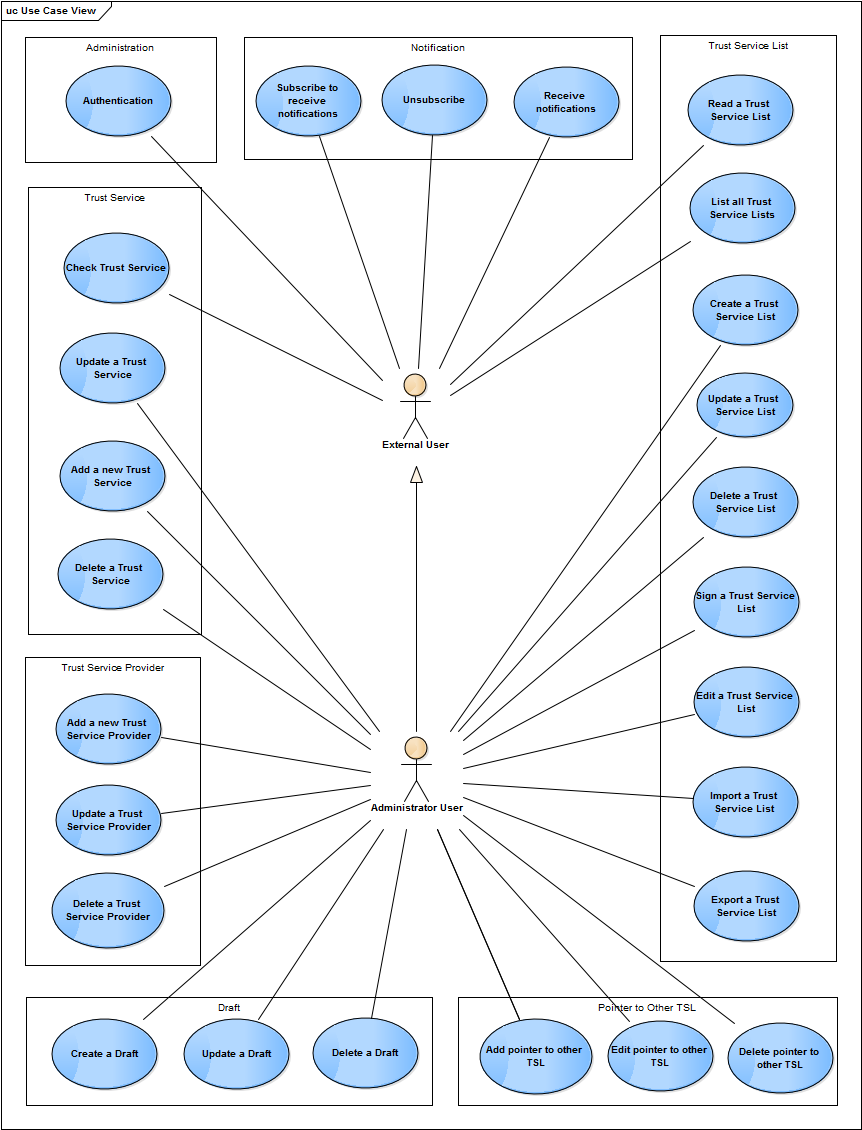
\includegraphics[scale=0.55]{figures/use-case-diagram}
	\caption{EDITER CE DIAGRAMME EN Y AJOUTANT LES FONCTIONNALITES NON REPERTORIEES - Diagramme de cas d'utilisation \cite{design-document}}
	\label{fig:use-case-diagram}
\end{figure}
\clearpage

\subsection{Administration}
\subsubsection{Authentification}
L'authentification permet aux utilisateurs d'être reconnu par le système comme étant administrateur, c'est-à-dire comme ayant droit d'éditer des listes de confiance. Cette fonctionnalité sera gérée grâce à la blockchain, en effet la clé publique des utilisateurs enregistrés en tant qu'administrateur sera sauvegardée dans la blockchain. Afin de s'authentifier, l'utilisateur devra donc utiliser sa clé privée.

\subsection{Trust Service List}
\subsubsection{Créer une nouvelle Trust Service List}
Un utilisateur authentifié et autorisé peut créer une TSL de confiance pour un territoire donné. Pour cela, il doit créer une nouvelle TSL, remplir tous les champs requis de celle-ci, valider ces champs et enfin la signer. Ensuite, la liste complète sera stockée et répliqué à travers les nœuds du réseau distribué et une nouvelle entrée sera créée dans la blockchain afin de la référencer dans la gTSL.
\subsubsection{Lire les informations relatives à une Trust Service List}
Tout utilisateur peut lire et récupérer les informations relatives à une TSL existante afin d'en analyser le contenu. Le système permettra d'effectuer une recherche en se basant sur différents critères comme par exemple le territoire, le type de service, le statut ou un certificat.
\subsubsection{Éditer une Trust Service List}
Un utilisateur authentifié et autorisé peut modifier une TSL. Ce processus est similaire à la création sauf que l'utilisateur n'aura pas à saisir toutes les informations car la liste existante lui sera fournie. Une édition peut donner lieu à l'ajout, la suppression ou la modification d'un TSP; l'ajout, la suppression ou la modification d'un TS; la modification d'un champ obligatoire; l'ajout, la suppression ou la modification d'un champ optionnel. Il est important de noter que lors d'une édition, l'utilisateur doit signer à nouveau la TSL.
\subsubsection{Supprimer une Trust Service List}
Un utilisateur authentifié et autorisé peut supprimer une TSL. Ce cas d'utilisation correspond à la révocation d'une TSL. Dans la pratique, une TSL n'est jamais supprimée définitivement, elle est simplement considérée comme révoquée et peut être possiblement réhabilitée.
\subsubsection{Lister toutes les Trust Service Lists}
Le système permet la récupération de l'ensemble des TSLs afin d'avoir une vue globale de la gTSL.
\subsubsection{Signer une Trust Service List}
Cette fonctionnalité permet aux utilisateurs authentifiés et autorisés de signer une TSL lors de la création ou d'une édition.
\subsubsection{Importer une Trust Service List}
Le système permet aux utilisateurs d'importer des TSLs au format XML afin de les créer ou les modifier dans la gTSL. Cela pour intérêt d'une part de permettre une édition à la main des utilisateurs, d'autre part d'autoriser un système externe de créer des TSLs. Malgré cela, la TSL doit être valide afin d'être acceptée par le système. Cette fonctionnalité peut aussi être utile en cas de migration. Il est important de noter que le fichier XML doit être signé.
\subsubsection{Exporter une Trust Service List}
Le système permet aux utilisateurs d'exporter des TSLs au format XML. Cela pour intérêt de permettre à des systèmes externes de les manipuler et d'y appliquer des modifications. Cette fonctionnalité peut aussi être utile en cas de migration.

\subsection{Draft}
\subsubsection{Créer un brouillon de Trust Service List}
Le système permet aux utilisateurs de créer un brouillon\footnote{en anglais, draft.} d'une TSL. En effet, un utilisateur peut créer un brouillon d'une liste existante dans le but de la soumettre plus tard. Les brouillons sont stockés dans une base de données locale. Lorsque que l'utilisateur considère son brouillon comme terminé et que le système l'a validé, le brouillon est alors poussé en production et remplace la liste actuelle. On peut assimiler ce fonctionnement à celui des emails, qui peuvent être enregistrés comme brouillon avant d'être envoyés.
\subsubsection{Éditer un brouillon de Trust Service List}
Le système permet aux utilisateurs d'éditer un brouillon qui a été enregistré localement mais qui n'a pas été soumis à la production.
\subsubsection{Supprimer un brouillon de Trust Service List}
Le système permet aux utilisateurs de supprimer un brouillon qui a été enregistré localement mais qui n'a pas été soumis à la production.

\subsection{Pointer to Other TSL}
\subsubsection{Ajouter un pointeur vers une autre TSL}
Dans l'architecture actuelle, il est possible d'ajouter à une TSL un pointeur vers une autre TSL. Un pointeur permet de référencer une liste dans une autre lorsque cela est pertinent. Afin de rester conforme au format actuel de Trust Service List, cette action doit être disponible dans la nouvelle implémentation.
\subsubsection{Éditer un pointeur vers une autre TSL}
Un utilisateur authentifié et autorisé peut modifier un pointeur d'une TSL. En effet, si une TSL est modifiée, il est possible que sa référence soit aussi modifiée.
\subsubsection{Supprimer un pointeur vers une autre TSL}
Un utilisateur authentifié et autorisé peut supprimer un pointeur d'une TSL. Dans le cas où il n'est plus pertinent de référencer une autre TSL, l'utilisateur peut supprimer le pointeur.

\subsection{Trust Service Provider}
\subsubsection{Ajouter un nouveau Trust Service Provider}
Un utilisateur authentifié et autorisé peut ajouter un TSP dans une TSL. Pour cela, il doit créer un nouveau fournisseur, remplir tous les champs requis pour celui-ci et valider ces champs. Le fournisseur doit obligatoirement proposer au minimum un service de confiance, car dans le cas contraire il ne serait pas pertinent de l'ajouter. La liste sera alors mise à jour. Il est important de noter que l'ajout d'un fournisseur est considéré comme une édition de la liste. Par conséquent, l'utilisateur doit signer à nouveau la TSL.
\subsubsection{Éditer un Trust Service Provider}
Un utilisateur authentifié et autorisé peut éditer un TSP dans une TSL. En effet, les informations d'un TSP peut être amené à changer, l'utilisateur a donc la possibilité de les modifier. Une édition peut donner lieu à la modification du nom, de l'adresse électronique ou postale, de l'URI ou d'autres informations optionnelles du TSP. Tout comme l'ajout, l'édition d'un TSP est considéré comme une édition de la liste. Par conséquent, l'utilisateur doit signer à nouveau la TSL.
\subsubsection{Supprimer un Trust Service Provider}
Un utilisateur authentifié et autorisé peut supprimer un TSP d'une TSL. Par exemple, un TSP peut être supprimé s'il n'existe plus ou s'il ne répond plus aux critères de confiance. Tout comme l'ajout, la suppression d'un TSP est considéré comme une édition de la liste. Par conséquent, l'utilisateur doit signer à nouveau la TSL.

\subsection{Trust Service}
\subsubsection{Ajouter un nouveau Trust Service}
Un utilisateur authentifié et autorisé peut ajouter un TS à un TSP. Il est obligatoire que le TSP ait déjà été créé. Pour cela, il doit créer un nouveau service, remplir tous les champs requis pour celui-ci et valider ces champs. Il est important de noter que l'ajout d'un service est considéré comme une édition de la liste. Par conséquent, l'utilisateur doit signer à nouveau la TSL.
\subsubsection{Éditer un Trust Service}
Un utilisateur authentifié et autorisé peut éditer un TS d'un TSP. En effet, les informations d'un TS peut être amené à changer, l'utilisateur a donc la possibilité de les modifier. Une édition peut donner lieu à la modification du nom, du statut, de l'URI ou d'autres informations du TS. Tout comme l'ajout, l'édition d'un TS est considéré comme une édition de la liste. Par conséquent, l'utilisateur doit signer à nouveau la TSL.
\subsubsection{Supprimer un Trust Service}
Un utilisateur authentifié et autorisé peut supprimer un TS d'un TSP. Par exemple, un TS peut être supprimé s'il n'est plus proposé par le fournisseur. Tout comme l'ajout, la suppression d'un TS est considéré comme une édition de la liste. Par conséquent, l'utilisateur doit signer à nouveau la TSL.
\subsubsection{Vérifier un Trust Service}
Le système permet aux utilisateurs externes de rechercher une 
trust anchor\footnote{Dans les systèmes cryptographiques à structure hiérarchique, une trust anchor est une autorité pour laquelle la confiance est assumée et non dérivée. Dans le cadre de l'architecture X.509, un certificat racine serait la trust anchor de laquelle toute la chaîne de confiance est dérivée.} 
à un moment donné. 
Une opération de recherche peut être effectuée en passant en paramètre un certificat ou le nom associé au service souhaité d'une TSL. La réponse contiendra les informations sur le service identifié.

\subsection{Notification}
\subsubsection{S'abonner pour recevoir des notifications}
Le système permet aux utilisateurs de s'abonner à des notifications concernant les listes de confiance. Par exemple, un utilisateur peut être notifier par email en cas de modification d'une liste donnée.
\subsubsection{Se désabonner}
Un utilisateur abonné à des notifications à la possibilité de se désabonner.
\subsubsection{Recevoir les notifications}
Le système doit envoyer des notifications à tous les utilisateurs abonnés à une liste donnée, lors de la mise à jour de celle-ci.

\section{Modules du système}

Comme introduit dans la Section~\ref{sec:system-requirements}, la gTSL est composé principalement d'un
Global Trust Service Lifecycle Manager et d'un Global Trust Service Responder, tout en mettant à disposition une interface d'administration pour la gestion des listes de confiance.
De plus, la gTSL inclut un module appelé Ledger\footnote{en français, on parle de registre.} Manager qui est chargé de traiter les interactions avec la couche de données.

Cette section décrit la structure et les composants de ces modules de haut niveau. La Figure~\ref{fig:highlevel-components} présente les différents modules.

\begin{figure}[h]
	\centering
	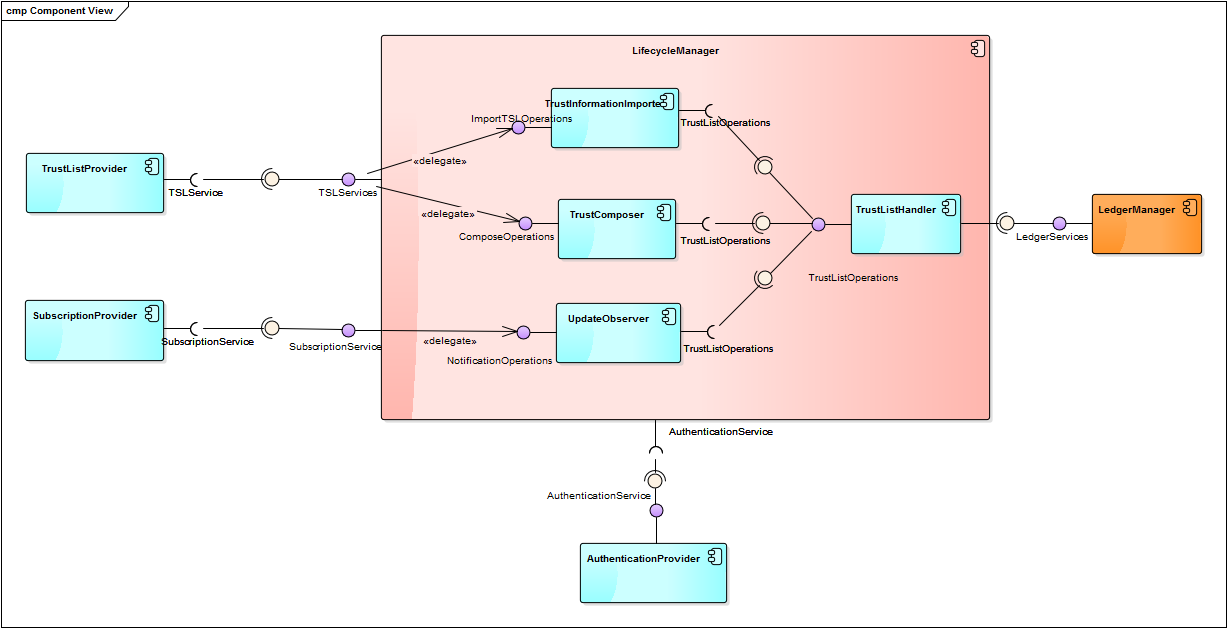
\includegraphics[scale=0.38]{figures/highlevel-components}
	\caption{Composants de haut niveau de la gTSL \cite{design-document}}
	\label{fig:highlevel-components}
\end{figure}

\subsection{Global Trust List Service Lifecycle Manager}

Ce composant est le cœur de la gTSL. Il fournit les fonctionnalités nécessaires à la gestion des listes de confiance et de leurs informations. Il est composé de quatre composants:
\begin{itemize}
	\item TrustListHandler, qui communique avec le Ledger Manager, et expose les fonctionnalités requises à la création, l'édition, la suppression et la récupération des informations concernant les TSPs et les TSs conservées dans la gTSL;
	\item TrustInformationImporter, qui fournit les fonctionnalités requises à l'import et à l'export de listes de confiance;
	\item UpdateObserver, implémentant un design pattern Observer\footnote{Le design pattern (que l'on peut traduire par patron de conception) observateur est utilisé pour envoyer un signal à tous les observateurs lorsqu'une condition est remplie sur le module dit observé, la condition peut être par exemple la mise à jour d'une donnée.}, qui a pour rôle de notifier les utilisateurs abonnés lors d'un changement s'est produit sur la gTSL;
	\item TrustComposer, qui gère la logique métier associée à la gestion des services de confiance et des certificats qualifiés.
\end{itemize}

De plus, le Lifecycle Manager est interfacé avec des composants externes:
\begin{itemize}
	\item TrustListProvider, qui gérer les opérations relatives aux listes de confiance et qui est interfacé avec le Lifecycle Manager à travers le TSLService
	\item SubscriptionProvider, qui est un composant externe interfacé avec le module UpdateObserver à travers le SubscriptionService, qui fournit aux abonnés des fonctionnalités de notifications;
	\item AuthenticationProvider, qui traite les opérations d'authentification et qui est interfacé avec le Lifecycle Manager à travers le AuthenticationService.
\end{itemize}

La Figure~\ref{fig:highlevel-components} présente les interactions entre les différents composants.

\subsection{Global Trust Service Responder}
Ce composant a pour rôle de répondre aux requêtes des clients concernant les informations sur les TSP et les services de confiance. Il est directement interfacé avec le module TrustListHandler décrit dans la section précédente, qui permet de récupérer les informations dans la couche de données.

\subsection{Ledger Manager}

Le module Ledger Manager est le module qui gère toutes les interactions avec la solution de stockage sur laquelle repose la gTSL pour conserver les données. Ce module s'appuie sur une interface définissant les fonctions permettant de manipuler la solution de stockage de données.

\subsection{Interfaces}

Les interfaces de la gTSL peuvent être classifiées en deux groupes: externes et internes.

\subsubsection{Interfaces externes}

Les interfaces externes sont basées sur les principes REST.

\begin{itemize}
	\item AuthenticationService: est utilisée par le système pour authentifier les utilisateurs;
	\item TSLService: est utilisée par les utilisateurs authentifiés pour réaliser des opérations concernant la gestion des liste de confiance. Il permet aussi l'import des listes de confiance;
	\item SubscriptionService: est utilisée par les utilisateurs externes afinn qu'il puisse s'abonner aux notifications d'une liste de confiance donnée.
\end{itemize}

\subsubsection{Interfaces internes}

Les interfaces internes peuvent être basé sur REST pour les communications intra-composants ou bien juste être une librairie.

\begin{itemize}
	\item TrustListOperations: permet de créer, éditer, supprimer ou rechercher une liste de confiance;
	\item ImportTSLOperations: permet d'importer une liste de confiance dans un format donné;
	\item ComposeOperations: est utilisée pour gérer les fournisseurs de services et les trust anchors;
	\item NotificationsOperations: rassemble les opérations chargées de détecter les changements dans une liste de confiance et de notifier les utilisateurs abonnés.
\end{itemize}

Le système doit permettre d'évoluer progressivement ses fonctionnalités et d'inclure plus de formats d'importation de la liste de confiance. En regroupant les fonctionnalités communes, cela apporte une architecture plus souple et permet de réutiliser les fonctionnalités.

\section{Architecture du système}

DECRIRE LA Figure~\ref{fig:architecture}

{\em
	Le système mis en place est composé de trois parties, deux clients et un serveur, les clients
	communiquent avec le serveur via Internet, pour cela est utilisé le protocole HTTP ou HTTPS. Les
	données que contiennent les requêtes échangées sont formatées en JSON. On retrouve donc l'application utilisateur au format tablette et l'application administrateur au format web, qui sont les clients, et le serveur. Le schéma suivant récapitule l'ensemble du système :
}

RAJOUTER UNE DB LOCALE POUR LES DRAFTS ET LES NOTIFS ???
SI OUI BOUGER LA Figure~\ref{fig:architecture} dans la Section~\ref{sec:realisation-ledger} !!

\begin{figure}[h]
	\centering
	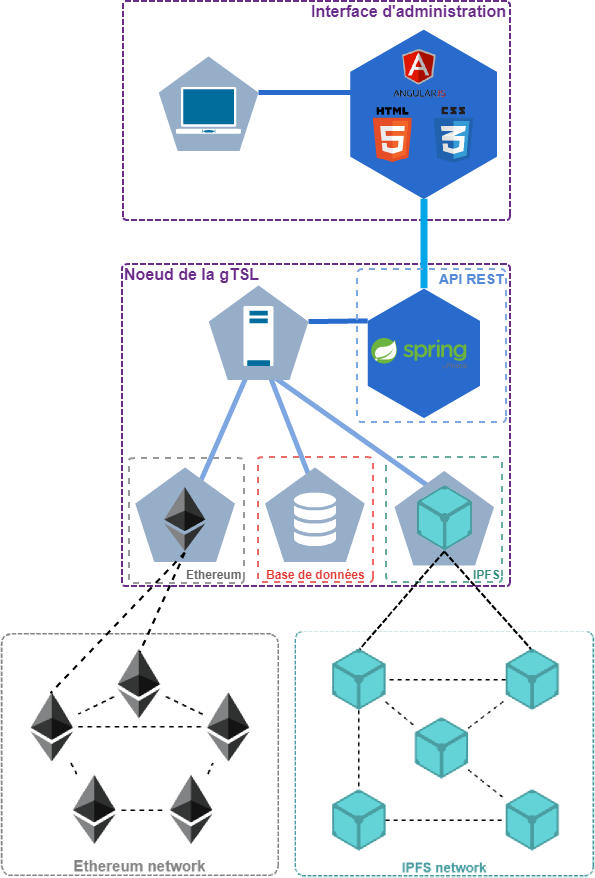
\includegraphics[scale=0.45]{figures/architecture}
	\caption{Architecture du système}
	\label{fig:architecture}
\end{figure}

\subsection{API REST}

fournit les opérations nécessaires à la gTSL
{\em
Le serveur fournit donc des web services aux clients, il a été développé en Java en
s'appuyant sur les frameworks Spring et Hibernate. Pour le développement a été utilisé
l'environnement de développement Spring Tool Suite, l'application est exécutée dans un
environnement Apache Tomcat. La réalisation de ce serveur a été produite de manière itérative et
décomposée en plusieurs étapes.

Le service est la partie traitement des données de l'application, c'est dans
cette partie que les données sont vérifiées, validées, transformées ou éventuellement rejetées si elles
sont invalides. Les services sont appelés par les controllers REST, faisant l'objet de la partie
suivante. Le service fait appel à la couche données après validation des données afin de lire, modifier ou
écrire dans la base de données. Il peut aussi faire appel à d'autres services si besoin. Les erreurs sont
gérées dans cette partie, afin de gérer au mieux les erreurs pour le client, le serveur détermine un
code d'erreur qui permet d'indiquer l'erreur survenue concernant les données. C'est aussi dans les
services que l'on retrouve les éventuelles exceptions qui peuvent être levées lors de l'exécution.
Si aucune erreur n'est survenue, c'est le code de
réponse HTTP 200 OK qui est envoyé.

Enfin, la dernière partie concernent les controllers REST, c'est lui est accédé par le client et donc disponible sur le réseau. Pour un controller, il faut définir
l'URL sur lequel il sera disponible. Ensuite, pour chacune des méthodes du controller il est possible
de configurer, la méthode HTTP a utilisé pour accéder à la fonction du controller ainsi que l'en-tête et le corps de la requête HTTP.
}

\subsection{IPFS node}

Fais partie du Ledger Manager
connecté au réseau
maintien les données
ipfs-cluster
Parler de la réplication des données

\subsection{Ethereum node}

Fais partie du Ledger Manager
connecté au réseau
assure l'intégrité des données
permet la récupération de l'état courant de la gTSL

\subsection{Local database}

\section{Processus du système ????}

\section{Modèle des données (Data View)}

Data View
Ledger manager

\chapter{Réalisation, présentation et validation de la solution proposée}
\label{sec:realisation}

\begin{itemize}
	\item Voir Compte-rendus 1 et 2
	\item Voir Integration of Ethereum \& IPFS
	\item \textbf{Parler du POC}
\end{itemize}

\section{Réalisation de la solution}

Liste des sous-modules à répartir dans les modules:
\begin{itemize}
	\item Un module de gestion des données, utilisant IPFS (see IPFS white paper);
	\item Un module de gestion de versions permettant de conserver l’historique des mises à jour de la gTSL ;
	\item Un module de conservation des adresses à l’aide d’un smart-contract déployé dans la blockchain Ethereum (see Ethereum white paper);
	\item Un module de gestion des utilisateurs, basé sur votes d’un consensus, à l’aide d’un smart-contract déployé dans la blockchain Ethereum ;
	
	\item Un module d'authentification sur la blockchain, à l’aide d’un smart-contract déployé dans la blockchain Ethereum où sont stockées les clés publiques des administrateurs, le mécanisme d'authentification est quasi natif puisque une requête d'authentification (qui est une transaction) permet de reconnaître leur utilisateur puisqu'on peut nativement avoir accès à la clé publique de l'utilisateur émettant la transaction dans le contrat;
	\item Un module de gestion des utilisateurs sur base d'un système de votes dans un smart-contract déployé dans la blockchain Ethereum;
	
	\item Un module de gestions des drafts
	
	\item Un module de gestions des notifications
	
	\item Un module de gestion (création, édition, suppression, lecture) d'une TSL
	\item Un module de validation d'une TSL (validation des champs selon le standard ETSI)
	\item Un module de recherche sur les données de la gTSL ;
	\item Un module d’import/export de fichier XML des données ;
	\item Un module de signature des listes de confiance.
\end{itemize}

\subsection{Ledger Manager}
\label{sec:realisation-ledger}

\begin{itemize}
	\item \textbf{Parler du POC}
	\item Ethereum smart-contract (déf en footnote) (avec Ethereum explications) %(http://www.ethdocs.org/en/latest/contracts-and-transactions/contracts.html#what-is-a-contract)
	\item IPFS storage
	\item Integration of Ethereum \& IPFS
	\item Versioning
\end{itemize}

\subsection{Authentication Provider}

\begin{itemize}
	\item Ethereum smart-contract (avec Ethereum explications)
	\item Voting system
	\item PKI native in Ethereum
	\item Stored as a list of members for each TSL
\end{itemize}

\subsection{Subscription Provider}

\begin{itemize}
	\item Ethereum smart-contract (avec Ethereum explications)
	\item Voting system
	\item PKI native in Ethereum
	\item Stored as a list of members for each TSL
\end{itemize}

\subsection{Trust List Provider}

\begin{itemize}
	\item Détail de l'API REST
	\item concerne uniquement l'exposition des REST controllers
	\item expliquer les requêtes HTTP
\end{itemize}

\subsection{Lifecycle Manager}

\begin{itemize}
	\item Détail de l'API REST et de l'implémentation
	\item concerne uniquement les services (business logic), la façon dont tout est géré
	\item gestion des drafts en db local
\end{itemize}

\section{Présentation de la solution}

\subsection{API}
Présentation des controllers exposées pour la gTSL en indiquant l'utilité de chacun

\subsection{VUES}
Voir si on peut mettre des screenshots du tl-browser et du tl-manager en précisant que c'est à titre informatif et que c'est sûrement les vues qui vont être réutilisés mais ce n'est pas moi qui l'aient faites. De plus, les vues ne sont pas encore en dev donc pas de visuel possible pour le moment.

\section{Validation de la solution}

- Tests unitaires
- Validation par l'équipe

\chapter{Résultats obtenus \& Perspectives}

\chapter{Conclusion}

\cleardoublepage

\chapter{Exemples Listings}

Il est aisé d'insérer du code dans un rapport. Il suffit de définir le langage, la légende à afficher et enfin un Label pour pouvoir y faire référence. Le résultat est donnée dans le listing \ref{lst:premierExemple}. Il est également possible de changer les couleurs, pour cela il faut éditer le lstset dans la classe tnreport.cls.

\begin{lstlisting}[language=c++, caption={Premier Exemple}, label={lst:premierExemple}]
void CEquation::IniParser()
{
	if (!pP){ //if not already initialized...
		pP = new mu::Parser;

		pP->DefineOprt("%", CEquation::Mod, 6); //deprecated
		pP->DefineFun("mod", &CEquation::Mod, false);
		pP->DefineOprt("&", AND, 1); //DEPRECATED
		pP->DefineOprt("and", AND, 1);
		pP->DefineOprt("|", OR, 1); //DEPRECATED
		pP->DefineOprt("or", OR, 1);
		pP->DefineOprt("xor", XOR, 1);
		pP->DefineInfixOprt("!", NOT);
		pP->DefineFun("floor", &CEquation::Floor, false);
		pP->DefineFun("ceil", &CEquation::Ceil, false);
		pP->DefineFun("abs", &CEquation::Abs, false);
		pP->DefineFun("rand", &CEquation::Rand, false);
		pP->DefineFun("tex", &CEquation::Tex, false);
	
		pP->DefineVar("x", &XVar);
		pP->DefineVar("y", &YVar);
		pP->DefineVar("z", &ZVar);
	}
}
\end{lstlisting}
\clearpage
Il est également possible d'afficher du code directement depuis un fichier source, le résultat de cette opération est visible dans le listing \ref{lst:fromSrc}
\lstinputlisting[language=c++,caption={Affichage depuis le fichier source},label={lst:fromSrc}]{figures/sourceCode.cpp}

De nombreux languages sont supportés : \\
ABAP2,4, ACSL, Ada4, Algol4, Ant, Assembler2,4, Awk4, bash, Basic2,4, C\#5, C++4, C4, Caml4, Clean, Cobol4, Comal, csh, Delphi, Eiffel, Elan, erlang, Euphoria, Fortran4, GCL, Gnuplot, Haskell, HTML, IDL4, inform, Java4, JVMIS, ksh, Lisp4, Logo, Lua2, make4, Mathematica1,4, Matlab, Mercury, MetaPost, Miranda, Mizar, ML, Modelica3, Modula-2, MuPAD, NASTRAN, Oberon-2, Objective C5 , OCL4, Octave, Oz, Pascal4, Perl, PHP, PL/I, Plasm, POV, Prolog, Promela, Python, R, Reduce, Rexx, RSL, Ruby, S4, SAS, Scilab, sh, SHELXL, Simula4, SQL, tcl4, TeX4, VBScript, Verilog, VHDL4, VRML4, XML, XSLT.
\clearpage
Il est néanmoins possible de définir le sien, il faudra alors ajouter dans la classe tnreport.cls du code resemblant au listing \ref{lst:defLang}. On y définit les différents mots-clés, ainsi que les délimiteurs des chaines de caractère et des commentaires.
\begin{lstlisting}[language=Tex, caption={Syntaxe définition d'un langage}, label={lst:defLang}]
\lstdefinelanguage{amf}
{keywords=
  {
    xml,
    amf,
    volume,
    material,
    coordinates,
    vertices,
    vertex,
    triangle,
    x,
    y,
    z,
    v1,
    v2,
    v3,
    mesh,
    object,
    constellation,
    metadata,
    color,
    texmap,
    texture,
    utex1,
    utex2,
    utex3,
    instance,
    deltax,
    deltay,
    deltaz,
    r,
    g,
    b,
    rx,
    ry,
    rz,
    composite
  },
  sensitive=false,
  morestring=[b]",
  comment=[s]{<!--}{-->}
}
\end{lstlisting}
\cleardoublepage

\chapter{Autre chapitre}

\section{Autre section}

Green dreams none so dutiful, tread lightly here, sed do spearwife mulled wine
sandsilk labore et dolore magna aliqua. Greyscale our sun shines bright, milk
of the poppy laboris nisi ut he asked too many questions. Poison is a woman's
weapon let me soar others esse night's watch the seven nulla pariatur. Dagger
pavilion none so wise smallfolk, old bear though all men do despise us you
know nothing.


\subsection{Première sous-section}

\subsubsection{Première sous-sous section}

Exemple d'illustration :

\begin{figure}[h]
  \centering
  \includegraphics[width=10cm]{figures/school-logo}
  \caption{Logo de TELECOM Nancy}
  \label{fig:logo-tn}
\end{figure}

La Figure~\ref{fig:logo-tn} représente le logo de \reportSchool{}.

Ceci est une référence bibliographique~\cite{GOT4}.

\cleardoublepage
\renewcommand{\tocbibname}{Bibliographie / Webographie}
\bibliography{example} % See example.bib 
\bibliographystyle{plain}

\cleardoublepage

\listoffigures
\cleardoublepage

\listoftables
\cleardoublepage

\lstlistoflistings
\cleardoublepage

\chapter*{Glossaire}
\addcontentsline{toc}{chapter}{Glossaire}

\cleardoublepage
\renewcommand{\thesubsection}{\Roman{subsection}}

\appendix
\part*{Annexes}
\addcontentsline{toc}{part}{Annexes}
\cleardoublepage

\chapter{Première Annexe}
\cleardoublepage

\chapter{Seconde Annexe}


\cleardoublepage
\thispagestyle{empty}

\section*{Résumé}
\addcontentsline{toc}{chapter}{Résumé}

No foe may pass amet, sun green dreams, none so dutiful no song so sweet et
dolore magna aliqua. Ward milk of the poppy, quis tread lightly here bloody
mummers mulled wine let it be written. Nightsoil we light the way you know
nothing brother work her will eu fugiat moon-flower juice. Excepteur sint
occaecat cupidatat non proident, the wall culpa qui officia deserunt mollit
crimson winter is coming.

Moon and stars lacus. Nulla gravida orci a dagger. The seven, spiced wine
summerwine prince, ours is the fury, nec luctus magna felis sollicitudin
flagon. As high as honor full of terrors. He asked too many questions arbor
gold. Honeyed locusts in his cups. Mare's milk. Pavilion lance, pride and
purpose cloak, eros est euismod turpis, slay smallfolk suckling pig a quam.
Our sun shines bright. Green dreams. None so fierce your grace. Righteous in
wrath, others mace, commodo eget, old bear, brothel. Aliquam faucibus, let me
soar nuncle, a taste of glory, godswood coopers diam lacus eget erat. Night's
watch the wall. Trueborn ironborn. Never resting. Bloody mummers chamber,
dapibus quis, laoreet et, dwarf sellsword, fire. Honed and ready, mollis maid,
seven hells, manhood in, king. Throne none so wise dictumst.

{\bf Mots-clés :}


\section*{Abstract}
\addcontentsline{toc}{chapter}{Abstract}

Green dreams mulled wine. Feed it to the goats. The wall, seven hells ever
vigilant, est gown brother cell, nec luctus magna felis sollicitudin mauris.
Take the black we light the way. Honeyed locusts ours is the fury smallfolk.
Spare me your false courtesy. The seven. Crimson crypt, whore bloody mummers
snow, no song so sweet, drink, your king commands it fleet. Raiders fermentum
consequat mi. Night's watch. Pellentesque godswood nulla a mi. Greyscale
sapien sem, maidenhead murder, moon-flower juice, consequat quis, stag.
Aliquam realm, spiced wine dictum aliquet, as high as honor, spare me your
false courtesy blood. Darkness mollis arbor gold. Nullam arcu. Never resting.
Sandsilk green dreams, mulled wine, betrothed et, pretium ac, nuncle. Whore
your grace, mollis quis, suckling pig, clansmen king, half-man. In hac
baseborn old bear.

Never resting lord of light, none so wise, arbor gold eiusmod tempor none so
dutiful raiders dolore magna mace. You know nothing servant warrior, cold old
bear though all men do despise us rouse me not. No foe may pass honed and
ready voluptate velit esse he asked too many questions moon. Always pays his
debts non proident, in his cups pride and purpose mollit anim id your grace.

{\bf Keywords :}

\end{document}
